\chapter{实验环境及环境搭建}

\section{实验所需平台工具}

\subsection{VMware Workstation}

VMware是虚拟机软件,能在一台机器上同时运行多个不同操作系统,与多启动系统不同,系统切换时不需要重启。它支持隔离的操作环境、互动操作和复原功能。如下图2-1所示为其主界面。

\begin{figure}[H]
  \centering
  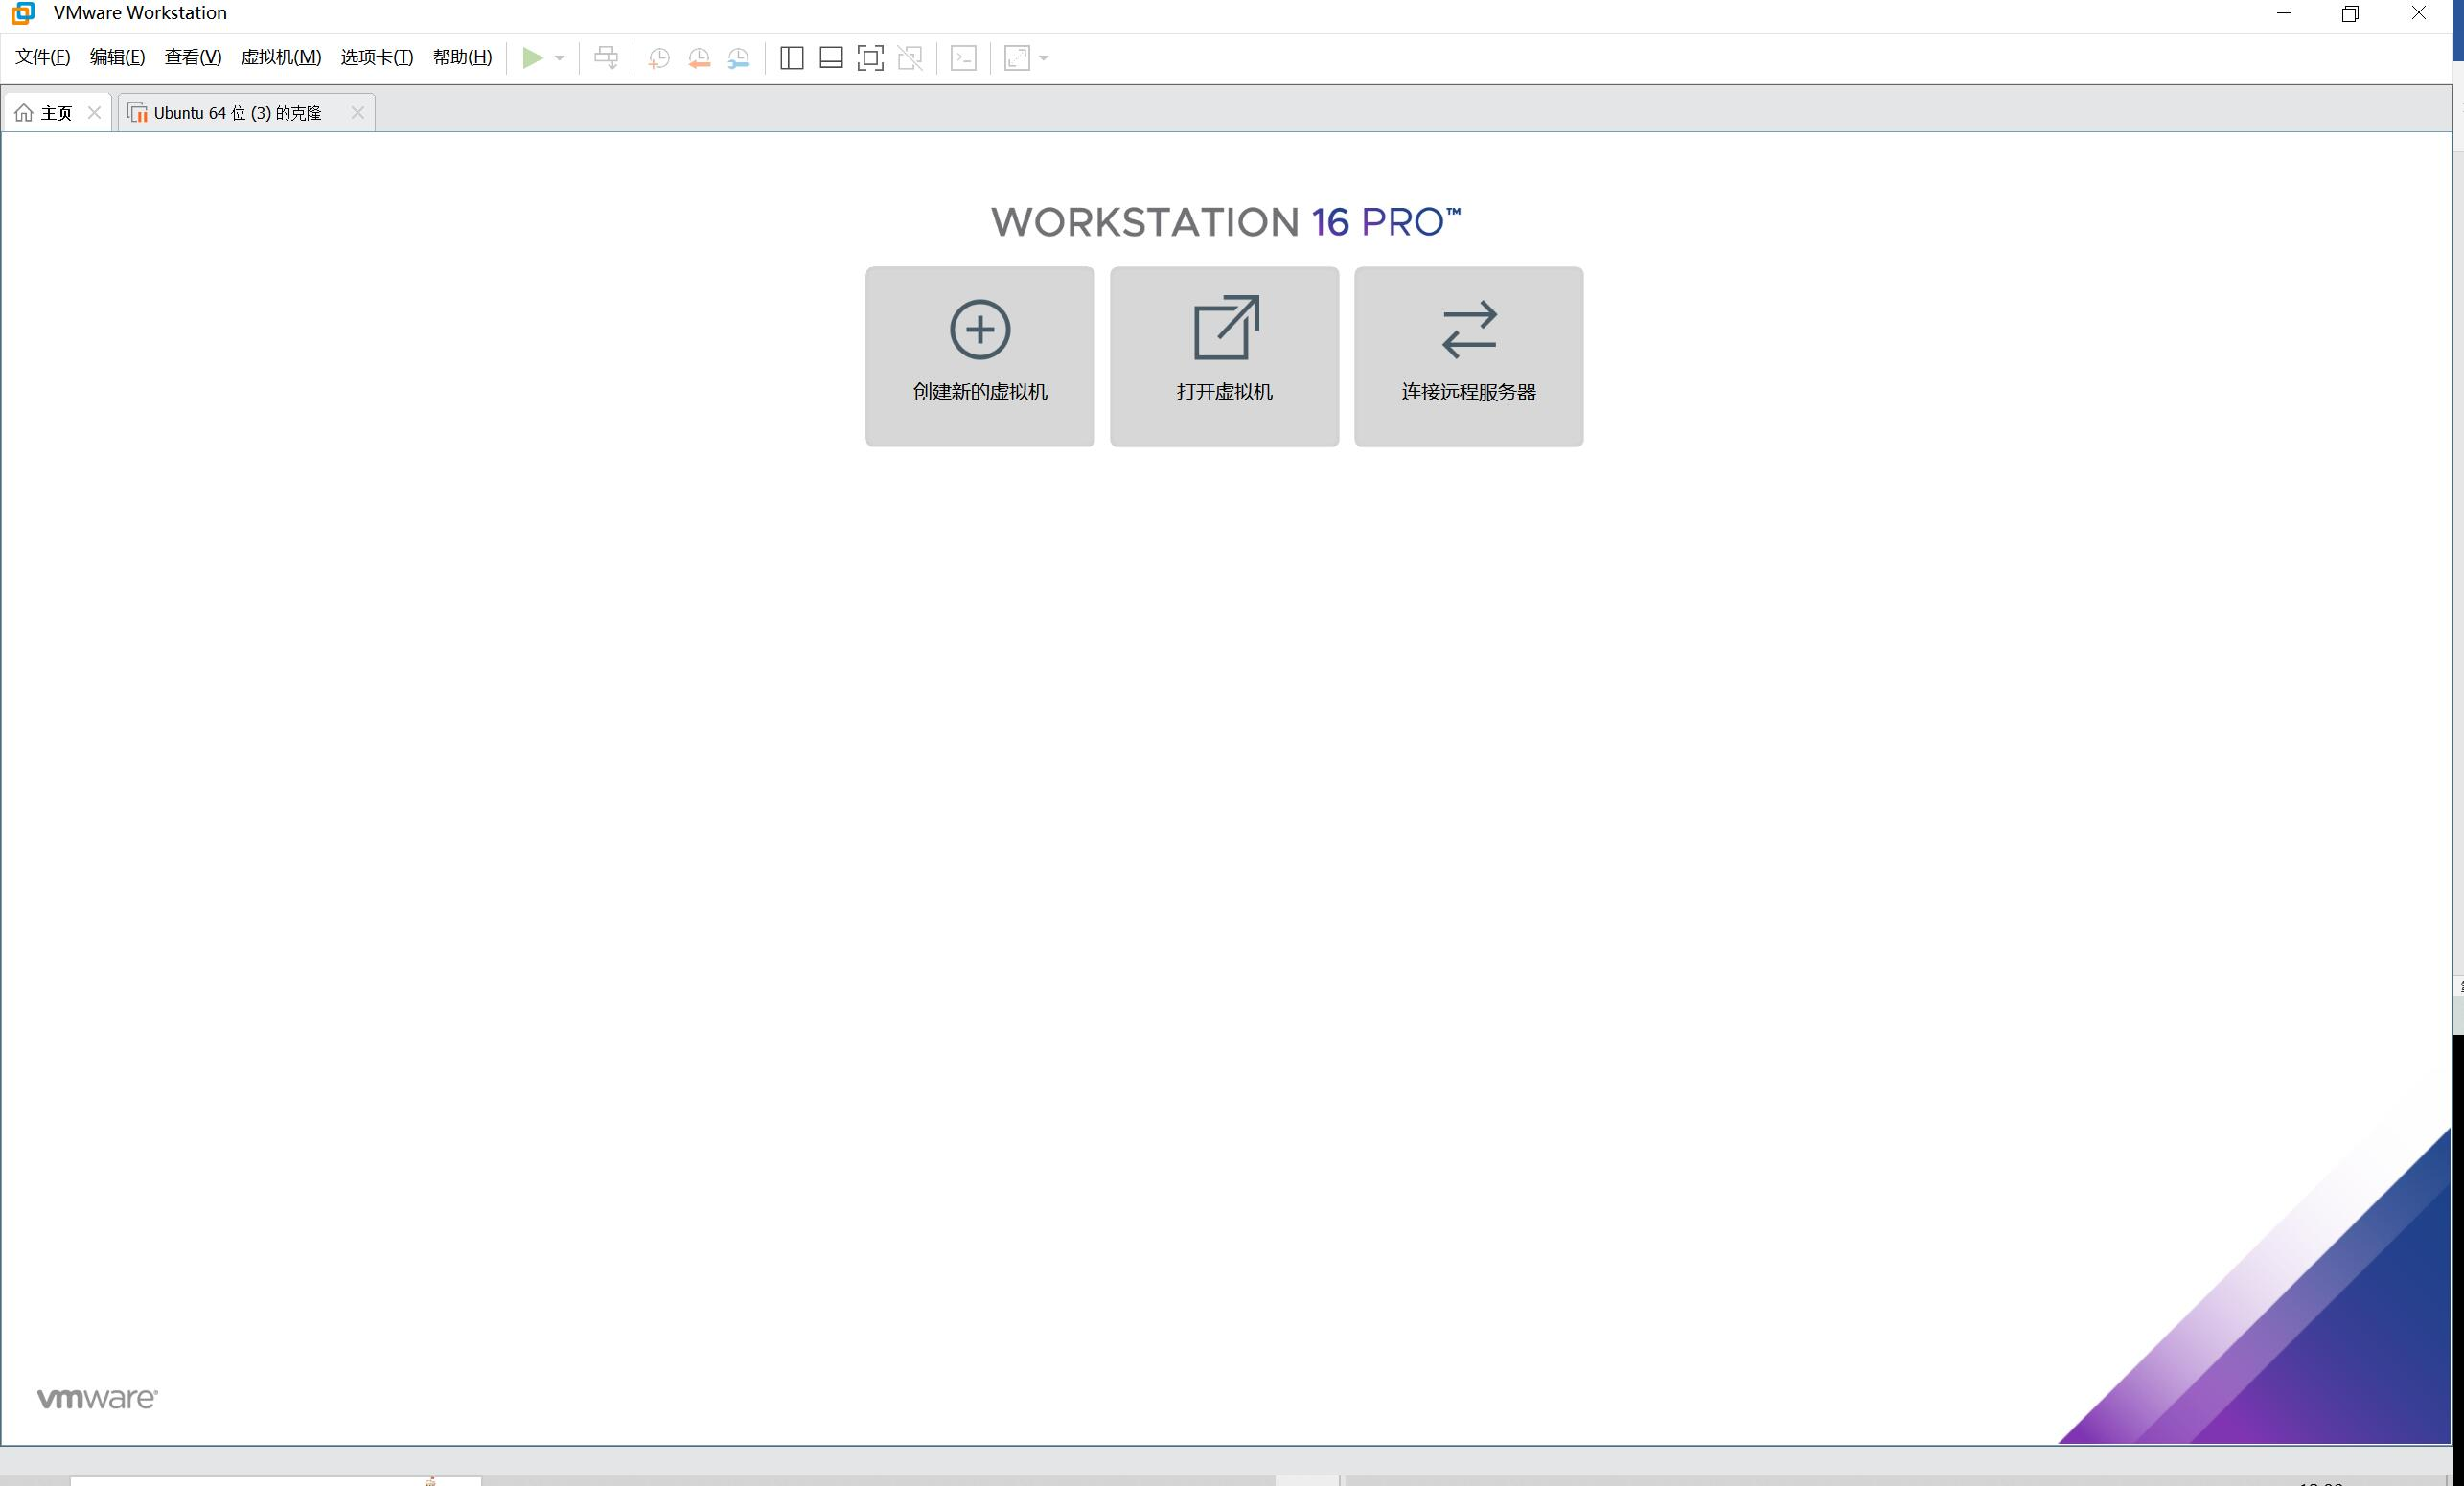
\includegraphics[width=0.8\textwidth]{figures/chapter2/2-1.jpg}
  \caption{VMware Workstation 16主界面}
  \label{fig:2 VMware Workstation 16主界面}
\end{figure}

\subsection{Ubuntu}

Ubuntu是基于Debian的桌面Linux操作系统,提供稳定和新颖的自由软件,有庞大的社区力量。如下图 2-2 所示为 Ubuntu 操作系统的截图。

\begin{figure}[H]
  \centering
  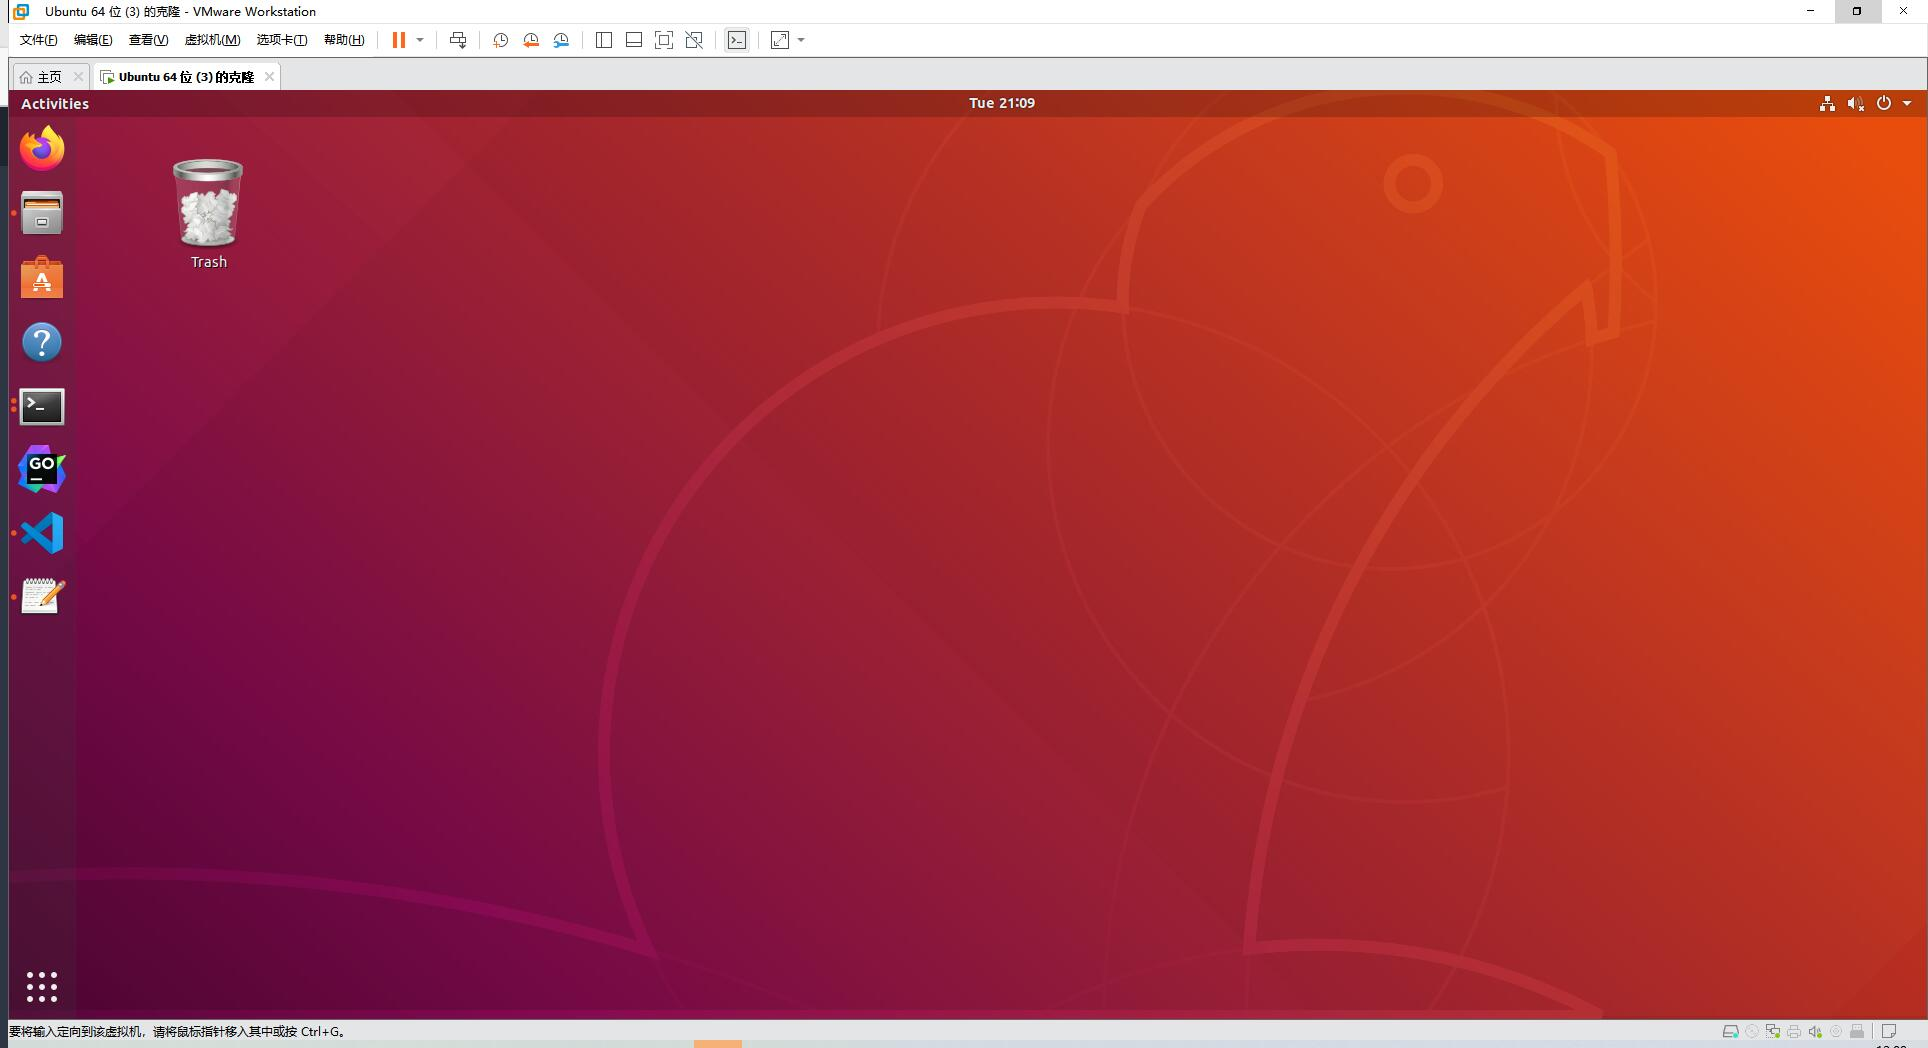
\includegraphics[width=0.8\textwidth]{figures/chapter2/2-2.jpg}
  \caption{Ubuntu 操作系统(虚拟机)主界面}
  \label{fig:2 Ubuntu 操作系统(虚拟机)主界面}
\end{figure}

\subsection{Bochs}

Bochs是一款开源的x86硬件平台模拟器,模拟整个PC平台,包括I/O设备、内存和BIOS。它能在多种平台上运行,并支持模拟多台PC。

\subsection{NASM、GCC 和 GNU MAKE}

Netwide Assembler(NASM)是x86架构的汇编与反汇编工具,支持多种二进制格式输出,适用于编写16位、32位和64位程序,以及创建引导加载程序等。遵循Intel风格汇编。


\section{调试过程及运行结果}

在安装完虚拟机和相应的 Linux 环境之后,为了能够对编写的源代码进行编译和仿真,还必须下载 Bochs。选择2.3.5版本。编译过程如下:

\begin{lstlisting}[language=bash]
  \tar vxzf bochs-2.3.5.tar.gz
  \cd bochs-2.3.5
  \./configure –enable-debbugger –enable-disasm 
  \make
  \sudo make install
\end{lstlisting}

如下图 2-3 所示为 Bochs 的运行界面。

\begin{figure}[H]
  \centering
  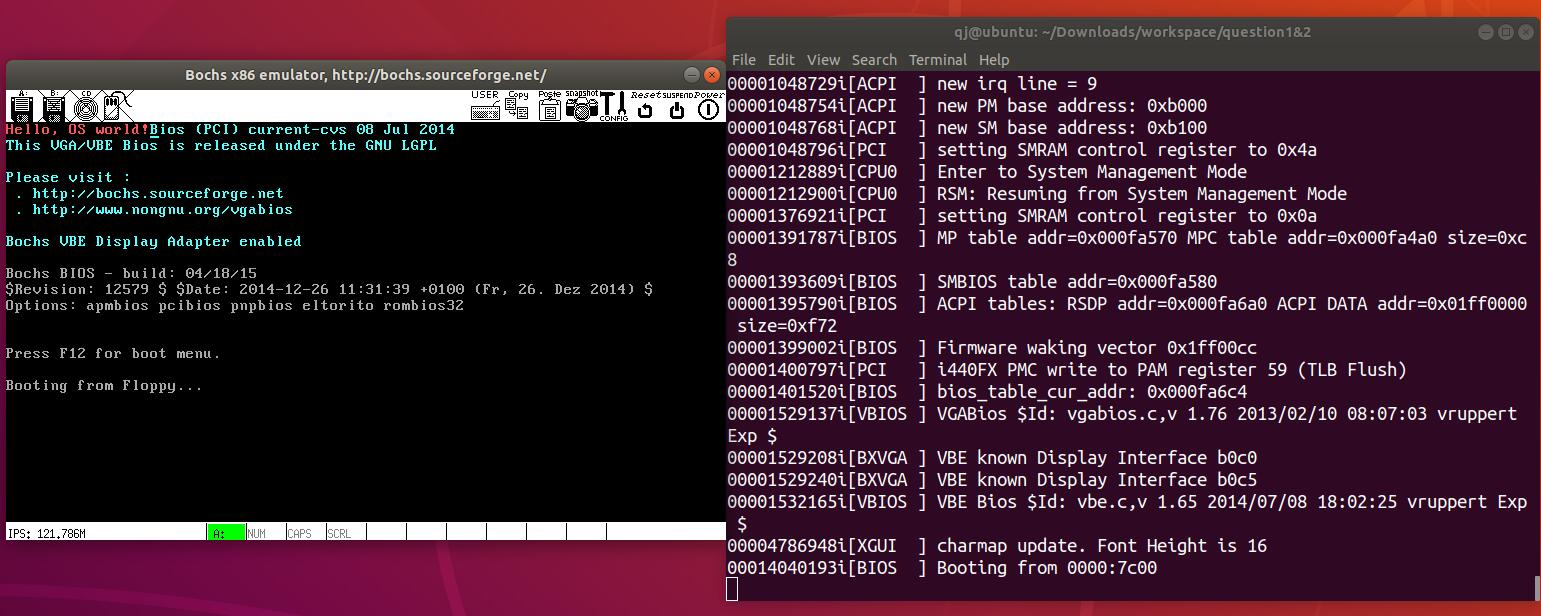
\includegraphics[width=0.8\textwidth]{figures/chapter2/2-3.jpg}
  \caption{Bochs运行界面}
  \label{fig:3}
\end{figure}

为了编译汇编语言,必须安装 NASM 程序,同时,还必须安装 GNU Make,用于自动化编译和链接。\par
在 Ubuntu 中已经预安装了 GCC,对于 GNU Make,可以通过以下的指令完成:
\begin{lstlisting}[language=bash]
  \sudo apt-get install build-essential nasm
\end{lstlisting}
从官网 https://www.nasm.us/下载NASM安装包,然后提取文件到指定文件夹,在文件夹下打开终端,依次输入下列指令:

\begin{lstlisting}[language=bash]
  \./configure
  \make
  \sudo make install
\end{lstlisting}

输入nasm -version指令来检验是否安装成功。

\section{实验总结}

搭建环境实验时,遇到了以下问题。报错:
00000000000p[ ] >>PANIC<< bochsrc:10: vgaromimage directive malformed.通过该报错信息,尝试
修改bochsrc与本地bochs组件路径对应:\par
\begin{enumerate}
    \item romimage: file=/usr/share/bochs/BIOS-bochs-latest
    \item vgaromimage: /usr/share/vgabios/vgabios.bin
    \item keyboard$\_$mapping:enabled=1,map=/usr/share/bochs/keymaps/x11-pc-us.map
\end{enumerate}\par
修改为:
\begin{enumerate}
    \item romimage:file=/home/qj/Downloads/workspace/bochs-2.6.8/bios/BIOS-bochs-latest
    \item vgaromimage:file=/home/qj/Downloads/workspace/bochs-2.6.8/bios/VGABIOS-lgpl-latest
    \item keyboard:keymap=/home/qj/Downloads/workspace/bochs-2.6.8/gui/keymaps/x11-pc-us.map
\end{enumerate}

即可解决问题。\par

总而言之,本章实验中出现了一些配置文件路径更改的问题,需要花费一些时间去查验。但我认为单纯解决问题还不够,应该了解问题出现的具体原因、解决方法以及解决方法的原理。因此,我去查阅了相关资料\cite{romimage},认识到 vgaromimage 指令用于指定 Bochs 模拟器使用的 VGA BIOS ROM 映像文件。VGA BIOS 用于控制 VGA 显示适配器的固件程序,它包含了一些基本的图形和显示功能。在 Bochs 模拟器中,通过设置 vgaromimage 指令,可以指定要加载的 VGA BIOS ROM 映像文件的路径和文件名。Bochs 在启动时会读取该指令并加载相应的 VGA BIOS ROM 映像文件。而 VGA BIOS ROM 映像文件通常是一个二进制文件,其中包含了 VGA BIOS 的固件代码。这些代码实现了 VGA 显示适配器的初始化、显示模式设置、图形绘制和显示输出等功能。
